\documentclass{beamer}

%\usepackage{beamerthemesplit}
\usepackage{graphicx}
%\usepackage{multicol}

\title{Turbulence Profiling}


\newcommand*{\captionsource}[2]{%
  \caption[{#1}]{%
    #1 %
    \hspace{\linewidth}%
%    \textbf{Source:} #2%
    Source: #2%
  }%
}


\newcommand{\tmean}[1]{\langle#1\rangle}
\newcommand{\abs}[1]{\left|#1\right|}


\newenvironment{wideitemize}{\itemize\addtolength{\itemsep}{15pt}}{\enditemize\hspace{\textwidth}}
\setbeamertemplate{bibliography item}{\insertbiblabel}

\begin{document}

\frame{\titlepage}
\section{Introduction}
\frame %<beamer:0>
{
	\frametitle{Fried parameter}
	\begin{itemize}
		\item Also called "seeing". 
		\item Defined as \cite{mohr2009atmospheric}
			\begin{align*}
				&r_0\equiv \left(0.423k^2\sec\zeta\int_{0}^{\infty} C_n^2(h)dh \right)^{-3/5} \left[length\right] 
			\end{align*}
			Where
			\begin{description}
				\item[$\displaystyle k=\frac{2\pi}{\lambda}$] the wave number $\displaystyle \left[length^{-1}\right]$
				\item[$\zeta$] The zenith angle
			\end{description}
		\item Describes the maximal resolution attainable by a telescope (with no correction for turbulence). 
	\end{itemize}
}
\frame
{
	\frametitle{Isoplanatic Angle \cite{roggemann1996imaging}}
	\begin{itemize}
		\item Defined by Fried 
	\end{itemize}
}
\frame[label={triangulation}]
{
	\frametitle{"Triangulation" principle (SCIDAR/SLODAR) 
	\cite{osborn2015characterising}}
       \begin{columns}
        \column{0.35\linewidth}
		\begin{figure}[l]
			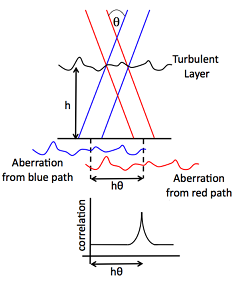
\includegraphics[width=1\textwidth]{images/scidar-triangulation.png}
			\caption{Triangulation with one turbulent layer. Source: 
			\cite{osborn2015characterising}}
		\end{figure}
	    \column{0.65\linewidth}
		    \begin{wideitemize}
			    \item Turbulence at height h illuminated by stars of	
			    angular separation $\theta$ produces two copies of the 
			    aberration separated by distance h$\theta$ 
			    \item Layer height extracted by cross correlating 
			    either centroid positions from a wavefront sensor 
			    (SLODAR) or intensity patterns (SCIDAR 
			    \cite{rocca1974detection},\cite{vernin1973experimental}) 
			\end{wideitemize} 
	
			(Originally, binary stars were used to have the images in the same 
			sensor \cite{vernin1973experimental}). 
		\end{columns}
}
\frame
{
	\frametitle{SCIDAR}
	\framesubtitle{Scintillation detection and ranging}
	\begin{itemize}
		\item Measured: irradiance $I(r, t)$
		\item Relative irradiance fluctuations: $\displaystyle X(r, t)=\frac{I(r, t)-\tmean{I(r, t)}}{\tmean{I(r, t)}}$
		\begin{itemize}
			\item Mean taken per-pixel over time - ergodicity assumed. 
		\end{itemize}
		\item Spatial autocovariance: 
		\begin{align*}
			C(\Delta r, \Delta t)=\tmean{X(r, t)X(r+\Delta r, t+\Delta t)}
		\end{align*}
		\item A turbulence layer at height $h$ (see slide \hyperlink{triangulation}{\ref{triangulation}}) produced by stars of angular separation $\theta$ yields two secondary peaks of $C$ at $\Delta r = \pm h\pmb{\theta}$ (\cite{rocca1974detection}, \cite{prieurthese})
	\end{itemize}
}
\frame 
{
	\begin{wideitemize}
	\item isoplanatic angle
	\end{wideitemize}
}
\frame
{
	\frametitle{Multi-Aperture Scintillation System (MASS)}
}
\frame 
{
	\frametitle{General facts}
	\begin{itemize}
	\item Turbulence is concentrated into thin layers
	\end{itemize}
}
\frame
{
	\frametitle{Acronyms}
	\begin{description}
		\item[DIMM] Differential image motion monitor
		\item[MASS] Multi aperture scintillation system
		\item[SCIDAR] Scintillation detection and ranging
		\item[TP] Turbulence profile
		\item[WFS] Wavefront sensor (Shack-Hartmann)
	\end{description}

	
}
%{
%	
%	\begin{figure} [ht]
%	  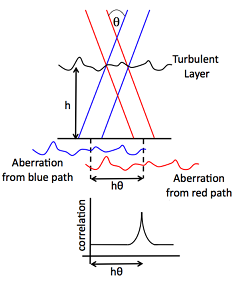
\includegraphics[width=0.5\textwidth]{images/scidar-triangulation.png}
%	  \centering
%	  \captionsource{}{\cite{osborn1a2013stereo}}
%	  \label{fig:gliederung}
%	\end{figure}
%}

\frame[allowframebreaks]
{
\bibliographystyle{plain}
\bibliography{survey}
}
\end{document}